% !TEX root = ../master-thesis.tex


\begin{figure}
    \centering
    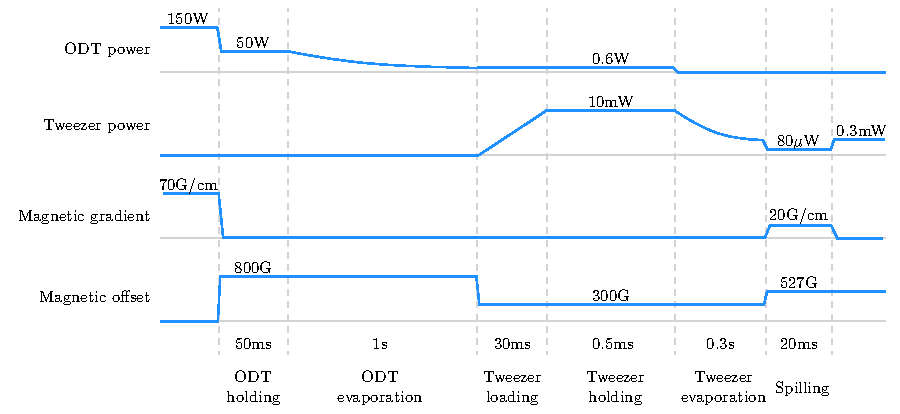
\includegraphics{fig-ai/preparation-seq.pdf}
    \caption[Experimental sequence for deterministic atom number preparation]{
        \textbf{Experimental sequence for deterministic atom number preparation.} 
        After loading a spin-balanced mixture into a crossed ODT from the MOT, we perform two-stage evaporation in the ODT. The atoms are then transferred into an optical tweezer via an adiabatic ramp. Further evaporation is carried out in the tweezer before executing the spilling procedure. Spilling takes place at 527\,G and a magnetic field gradient of 20\,G/cm to remove atoms above the spill level. The full sequence enables high-fidelity few-body preparation within a sub-2\,s cycle time. A detailed description can be found in~\cite{culemann_construction_2024}.
    }
    \label{fig:preparationseq}
\end{figure}


% \textbf{Beam collimation and polarization.} 
The tweezer array is formed by delivering light from a fiber outcoupler and collimating it with an achromatic lens mounted on a translation stage for precise control \cite{culemann_construction_2024}. To ensure efficient diffraction through the acousto-optic deflectors (AODs), horizontal polarization is set using a $\lambda/2$ waveplate and a polarizing beam splitter (PBS). Correct alignment of the PBS is verified by tracking the beam position on a camera before and after insertion.

% \textbf{Acousto-optic deflectors and relay imaging.} 
The array is generated using a pair of orthogonally mounted AODs, each mounted on custom blocks to maintain a common beam height of 100\,mm. The beam is guided into the first AOD using two mirrors, and its alignment is optimized to maximize both transmission and diffraction efficiency (typically exceeding 90\% at 65\,MHz). The two AODs are connected via a 4f relay built from achromatic lenses (Fig. \ref{fig:control}a). Precise positioning is achieved by aligning the relay externally using collimated light and checking for minimal wavefront distortion on a shear plate. An iris at the Fourier plane of the relay filters out the zeroth diffraction order.

% \textbf{Telescope and beam expansion.}
After the second AOD, the beam is expanded using a telescope consisting of two lenses. 
% $f = 150\,\mathrm{mm}$ and $f = 500\,\mathrm{mm}$
% The alignment ensures that the beam is collimated and centered on both lenses. The position of the second lens is mechanically fixed, while the telescope length is adjusted via mirror positions to achieve good collimation, verified with a shear plate. 
The zeroth-order beam after the second AOD is blocked at the intermediate focus.
% \textbf{Monitoring and power balancing.} 
A flip mirror is installed in the beam path to optionally redirect the light into a monitoring camera without disturbing the main optical alignment. This enables fast access to the tweezer array profile during alignment or balancing procedures.

We avoid using a back-side polished mirror for beam sampling in front of the camera. Although commonly employed for its simplicity, such mirrors introduce spatially varying interference fringes due to reflections from different internal surfaces of the substrate. These fringes distort the measured intensity distribution, especially for rays entering the camera at different angles and positions. This effect becomes critical when calibrating the response of the AODs, as it leads to systematic errors in measured beam uniformity. Instead, we sample the beam with a removable flip mirror that fully redirects the beam, ensuring an undistorted and angle-independent intensity profile at the camera plane.



